\chapter{Il recupero ed il salvataggio dei dati multimediali}

I file multimediali rappresentano un elemento centrale 
all’interno di un’applicazione orientata alla condivisione sociale,
contribuendo significativamente all’esperienza utente e all’interazione tra i partecipanti.
La possibilità di acquisire e condividere contenuti visivi, come immagini e video, 
consente di documentare eventi e attività,
favorendo una memoria collettiva e rafforzando il legame tra gli utenti.
In particolare, l’integrazione di materiale multimediale associato a eventi condivisi 
permette di preservare una rappresentazione più completa e dettagliata dell’esperienza vissuta,
migliorando l’engagement e la partecipazione all’interno della piattaforma, 
rappresentando uno dei punti di forza dell’applicazione.\\
\\
Tuttavia, la gestione dei file multimediali introduce complessità operative 
sia per il sistema sia per gli utenti stessi.
Da un lato, la selezione e l’invio dei contenuti 
possono rappresentare un onere significativo per l’utente, 
aumentando l’attrito nell’utilizzo dell’applicazione.
Per ottimizzare il processo e migliorare l’usabilità, 
è essenziale semplificare al massimo l’interazione richiesta,
automatizzando il recupero dei dati e limitando il ruolo dell’utente 
alla semplice conferma dei contenuti selezionati.
Questo approccio non solo semplifica l’esperienza d’uso, 
ma la rende più intuitiva e fruibile,
contribuendo anche a un incremento del tasso di adozione e della frequenza di utilizzo dell’applicazione.\\
\\
Parallelamente, la memorizzazione e il trasferimento di file multimediali 
pongono sfide significative a livello infrastrutturale,
in quanto tali dati presentano un impatto rilevante 
sulle risorse computazionali e sulla gestione dello storage.
Il volume elevato di richieste di caricamento e accesso ai file 
può infatti compromettere le prestazioni del sistema,
introducendo ritardi causati dal traffico di azioni 
che potrebbero influire negativamente sulle altre operazioni dell’applicazione.
Per garantire un’archiviazione efficiente e scalabile, 
è quindi necessario implementare una strategia di gestione della memoria
che separi il salvataggio dei file multimediali dal database principale, 
evitando di sovraccaricare il server applicativo.
Questa soluzione deve inoltre garantire un aggiornamento tempestivo delle informazioni, 
assicurando la sincronizzazione tra i dati archiviati e le modifiche effettuate dagli utenti.\\
\\
Per affrontare tali problematiche, 
un primo esame osserverà le modalità di recupero dei file multimediali,
con un focus sulle tecniche di selezione e rilevamento automatico delle immagini, 
nonché sui vincoli normativi e di sicurezza che ne regolano l’utilizzo.
In un secondo tempo l’analisi si concentrerà invece 
sulle strategie di salvataggio e gestione dello storage,
analizzando le diverse tipologie di archiviazione disponibili e le soluzioni implementate 
per garantire scalabilità, efficienza e riduzione dell’impatto sulle prestazioni del sistema.\\

\section{Le modalità di recupero delle immagini }

L’aggiunta di immagini a un evento prevede una fase preliminare di recupero, 
che consente all’utente di selezionare i file multimediali da associare. 
Il sistema offre due modalità principali di acquisizione: 
la selezione manuale da parte dell’utente, 
che può scegliere le immagini direttamente dalla memoria del dispositivo, 
e in alternativa, disponibile sui dispositivi mobili, un meccanismo automatizzato, 
che identifica le foto scattate durante lo svolgimento dell’evento.\\
\\
L’implementazione di questa funzionalità automatica di analisi della galleria 
per individuare i file multimediali desiderati  richiede l’accesso alla galleria fotografica del dispositivo, 
un’operazione subordinata al consenso esplicito dell’utente. 
Per questo motivo, al primo avvio dell’applicazione, 
il sistema richiede l’autorizzazione per accedere ai file multimediali, 
unitamente al permesso per la gestione delle notifiche. 
Nel caso in cui l’utente neghi l’accesso 
la richiesta verrà riproposta ogni qualvolta il sistema rilevi la necessità 
di accedere alla galleria per il recupero delle immagini.\\
\\
Al termine di ogni evento, non appena possibile, 
l'applicazione avvia automaticamente un’analisi della galleria locale, 
individuando le immagini scattate durante tutta la durata dell’evento. 
Se il sistema rileva la presenza di contenuti pertinenti, 
ne memorizza temporaneamente i riferimenti in una memoria locale per poi inviare una notifica all’utente, 
informandolo del ritrovamento delle immagini. 
A questo punto, l’utente ha la possibilità di esaminare le immagini suggerite, 
escluderne alcune o confermarne l’intero set per il caricamento.\\
\begin{figure}[htb]
    \centering
    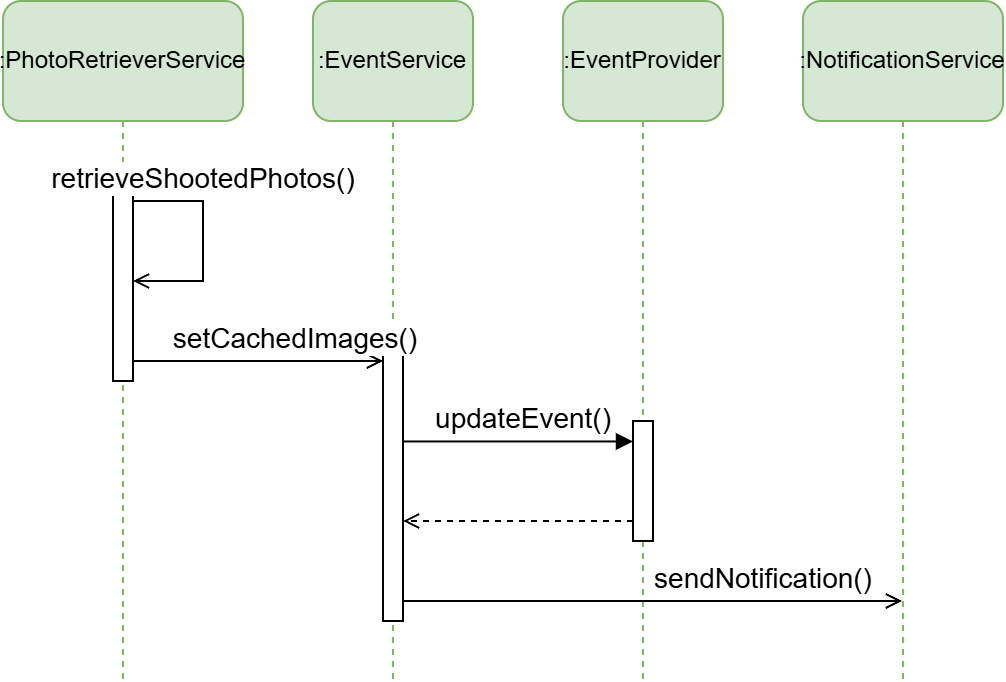
\includegraphics[height=0.45\textheight]{IIRecuperaImmagini.png}
    \caption{Interazione tra i componenti per il recupero delle immagini}
\end{figure}
\clearpage
Questa fase di conferma, oltre a garantire la trasparenza del servizio nei confronti dell’utente, 
riducendo il rischio di errori o caricamenti indesiderati, 
presenta anche vantaggi in termini di ottimizzazione delle prestazioni. \\
\\
Da un punto di vista normativo, 
la procedura di recupero e selezione automatica delle immagini
è esplicitamente descritta nelle condizioni d’uso dell’applicazione, 
alle quali l’utente deve aderire con accettazione espressa prima di utilizzare il servizio. 
Tuttavia, la fase di conferma dell’utente non rappresenta un obbligo giuridico, 
poiché la responsabilità della pubblicazione di contenuti multimediali 
ricade sul soggetto che realizza la fotografia. 
In conformità con la normativa vigente in materia di tutela dell’immagine 
(art. 10 c.c. e artt. 96-97 della Legge n. 633/1941) e protezione dei dati personali (Regolamento UE 2016/679 – GDPR), 
chi scatta una fotografia è tenuto a ottenere il consenso delle persone ritratte 
prima di procedere alla sua pubblicazione.\\
\\
Come già affrontato nel capitolo precedente, 
le operazioni che coinvolgono la modifica di uno stesso componente del sistema 
sono soggette a vincoli di concorrenza per l’accesso alla risorsa di interesse. 
La conclusione di un evento condiviso tra più utenti 
potrebbe generare richieste simultanee per l’aggiunta di immagini associate a un medesimo evento. 
L’introduzione della fase di selezione introduce un ritardo nella fase di caricamento, 
dilatando la distribuzione temporale delle richieste e riducendo la probabilità di collisioni 
dovute a operazioni concorrenti sullo stesso elemento.
L’attesa della conferma dell’utente prevede infatti un ritardo fisiologico 
tra la fine dell’evento e l’effettivo caricamento delle immagini, 
contribuendo a distribuire le richieste nel tempo e 
limitando il rischio di congestione del server, 
dovuta a operazioni simultanee su un singolo evento.\\
\\
Una volta completata la selezione da parte dell’utente, 
le immagini devono essere salvate sul server, 
per essere rese disponibili anche agli altri profili con cui l'evento è condiviso.
\clearpage
\section{L'integrazione con il sistema}

A differenza dei dati usualmente scambiati all'interno del sistema, 
i file multimediali presentano dimensioni significativamente superiori, 
con una differenza che si manifesta su ordini di grandezza rilevanti. 
Salvare questi file nella stessa modalità degli altri dati, 
affiancandoli quindi agli elementi logici, 
comporterebbe un impatto significativo sulla dimensione totale del database,
andando a influenzare tutte le operazioni eseguite su di esso,
che dovrebbero recuperare informazioni su un volume di dati molto più vasto del necessario.
Il rallentamento generale delle operazioni comporterebbe
un impatto significativo sulle prestazioni complessive del sistema.
Per questo motivo, è necessaria una gestione della memoria 
specificamente progettata per l'archiviazione e il recupero di contenuti multimediali.\\
\\
Inoltre, le dimensioni delle immagini e dei video influenzano direttamente 
il tempo di elaborazione e il volume delle richieste, 
aumentando il carico computazionale su tutti i componenti del sistema. 
Infatti la possibilità di allegare più file a un singolo evento implica 
che i tempi di caricamento elevati dei file multimediali 
possano prolungare sensibilmente la durata delle transazioni necessarie per la modifica degli eventi, 
incidendo sulla reattività del sistema.\\
\subsection{La scelta del servizio di persistenza}

La visualizzazione dei file multimediali riveste un'importanza secondaria
rispetto ad altre funzionalità offerte dall'applicazione.
Di conseguenza, è possibile accettare un maggiore tempo di caricamento, 
a condizione che ciò contribuisca a ridurre la latenza delle operazioni invece più rilevanti. 
Il salvataggio dei file multimediali direttamente nel database centrale 
comporterebbe un aumento significativo del volume delle richieste, 
determinando un maggiore impiego di risorse computazionali e un incremento dei tempi di caricamento. 
Questo fenomeno potrebbe incidere negativamente sulle prestazioni complessive del sistema, 
penalizzando l'esecuzione simultanea di altre operazioni.\\
\\
Per ottimizzare la gestione dei file multimediali, 
si è deciso di distinguere il dato binario dalla sua rappresentazione logica. 
In questo modo, la relazione tra il file e l'evento associato può essere mantenuta 
indipendentemente dai dati binari che lo compongono. 
Una volta recuperati i riferimenti logici ai file multimediali associati all'evento interessato, 
sarà possibile ottenere in un secondo momento i loro contenuti binari in un secondo momento, 
solo quando necessario.
Il modello del dominio illustrato in precedenza evidenzia 
la relazione logica tra gli eventi e i file associati (Image).\\
\\
Considerando la necessità e la possibilità di archiviare i file multimediali 
su risorse differenti dal database centrale, 
è fondamentale individuare la soluzione più adatta per la loro persistenza. 
I principali servizi cloud per l'archiviazione di file multimediali si suddividono in tre categorie: 
Object Storage, File Storage e Block Storage.\\
\\
Gli Object Storage gestiscono i file in un unico livello, 
con la possibilità di aggiungere metadati agli oggetti. 
A ciascun elemento viene associato un identificativo univoco che ne consente il recupero. 
L'accesso ai dati avviene tipicamente tramite API RESTful, 
che oltre a offrire la possibilità di gestire i permessi, 
garantisce l'utilizzo su ampia scala. 
La presenza di un unico livello di indirizzamento permette una scalabilità pressoché illimitata, 
e un costo variabile in base alla quantità di dati memorizzati.\\
\\
I File Storage organizzano i file in una struttura gerarchica di cartelle e sottocartelle, 
semplificando la gestione dei file e il controllo degli accessi. 
Oltre a facilitare un controllo ulteriore agli utenti, 
questa soluzione è compatibile con protocolli di accesso particolari. 
Tuttavia, la sua capacità e scalabilità, così come il costo effettivo, 
sono legati alla struttura dei file e alla capacità prevista dal piano selezionato.\\
\\
Infine, i Block Storage gestiscono la memoria tramite la suddivisione dei dati in blocchi logici,
salvati separatamente e ognuno dotato di identificativo univoco. 
Questa tecnologia offre elevate prestazioni per il recupero e la modifica dei dati, 
ma i costi aumentano all'incremento della quantità di dati presenti. 
La scalabilità è quindi limitata alla capacità assegnata al volume. 
Oltretutto, i costi sono elevati, particolarmente nel caso di grandi moli di dati.\\
\\
Tra queste soluzioni, 
la categoria degli Object Storage risulta la più adatta alle esigenze del progetto di salvataggio dei file multimediali. 
La sua scalabilità illimitata consente di gestire grandi volumi di elementi 
con una ridotta dipendenza tra loro. 
Inoltre, l'identificazione univoca di ciascun oggetto garantisce una rapida individuazione dei dati e 
un'efficiente risposta prestazionale a numerose richieste contemporanee.\\
\\
\begin{wrapfigure}{r}{0.25\textwidth}
    \centering
    
\includegraphics[height=.12\textheight]{blobstorage.png}
    Azure Blob Storage
\end{wrapfigure}
Nel contesto di Azure, 
il servizio di Object Storage fornito è rappresentato da Azure Blob Storage (ABS). 
ABS adotta un'organizzazione centrata su container, 
entità logiche che raggruppano più file multimediali e introducono un livello di indirizzamento aggiuntivo. 
L'accesso in lettura ai dati avviene tramite protocollo API RESTful, 
con autenticazione per l'aggiunta di nuovi elementi. 
I container creati sono relativi alle categorie per le quali le immagini vengono salvate.
Ad esempio, ci sarà un container relativo alle immagini degli eventi,
così come uno per quelle legate ai profili.\\
\\
All'interno del nome del blob si possono però aggiungere percorsi logici, 
separati dal carattere "\textbackslash".
Le immagini vengono quindi identificate univocamente attraverso la combinazione 
del container, dell'hash dell'elemento a cui fanno riferimento(l'evento, il profilo...) 
e del loro hash, concatenati per formare il percorso finale in cui sarà possibile recuperarle.\\
\\
\subsection{La procedura di salvataggio}

Una volta inizializzato Azure Blob Storage, le Azure Functions potranno connettersi per 
creare e gestire i container.
La richiesta parte dal client verso le Azure Functions, 
a seguito della selezione dei file multimediali da parte dell'utente.
La richiesta include, oltre all'hash dell'evento interessato, la lista delle estensioni dei file che si vuole salvare.\\
\\
Ricevuta la lista delle estensioni, 
la funzione chiamata esegue una verifica dei permessi di accesso necessari,
per poi connettersi a Cosmos DB, 
dopo aver controllato che le estensioni siano tra quelle accettate dal sistema,
essersi accertato che l'evento esista e aver generato gli hash per le future immagini.
Inserisce quindi nel database i nuovi riferimenti logici alle immagini,
che includono, oltre al loro hash, il riferimento all'evento, la loro estensione
e lo stato di elaborazione, inizializzato a "Created".
Si connette quindi ad Azure Blob Storage per ottenere un Shared Access Signarure (SAS) token.\\
\\
Il SAS token è un codice che viene usato per fornire permessi su servizi a entità terze.
Chiunque sia in possesso del token ha la possibilità di eseguire le modifiche a esso collegate. 
È infatti possibile definire i permessi, la durata e la località da associare al token.
In particolare, essendo le immagini salvate in un percorso logico che segue l'evento,
il token richiesto dalla funzione e generato dal ABS 
avrà la possibilità di creare e scrivere file sul container "eventi", 
nel percorso dell'evento corrispondente.
La validità di utilizzo ha durata dieci minuti.\\
\begin{figure}[h!]
    \centering
    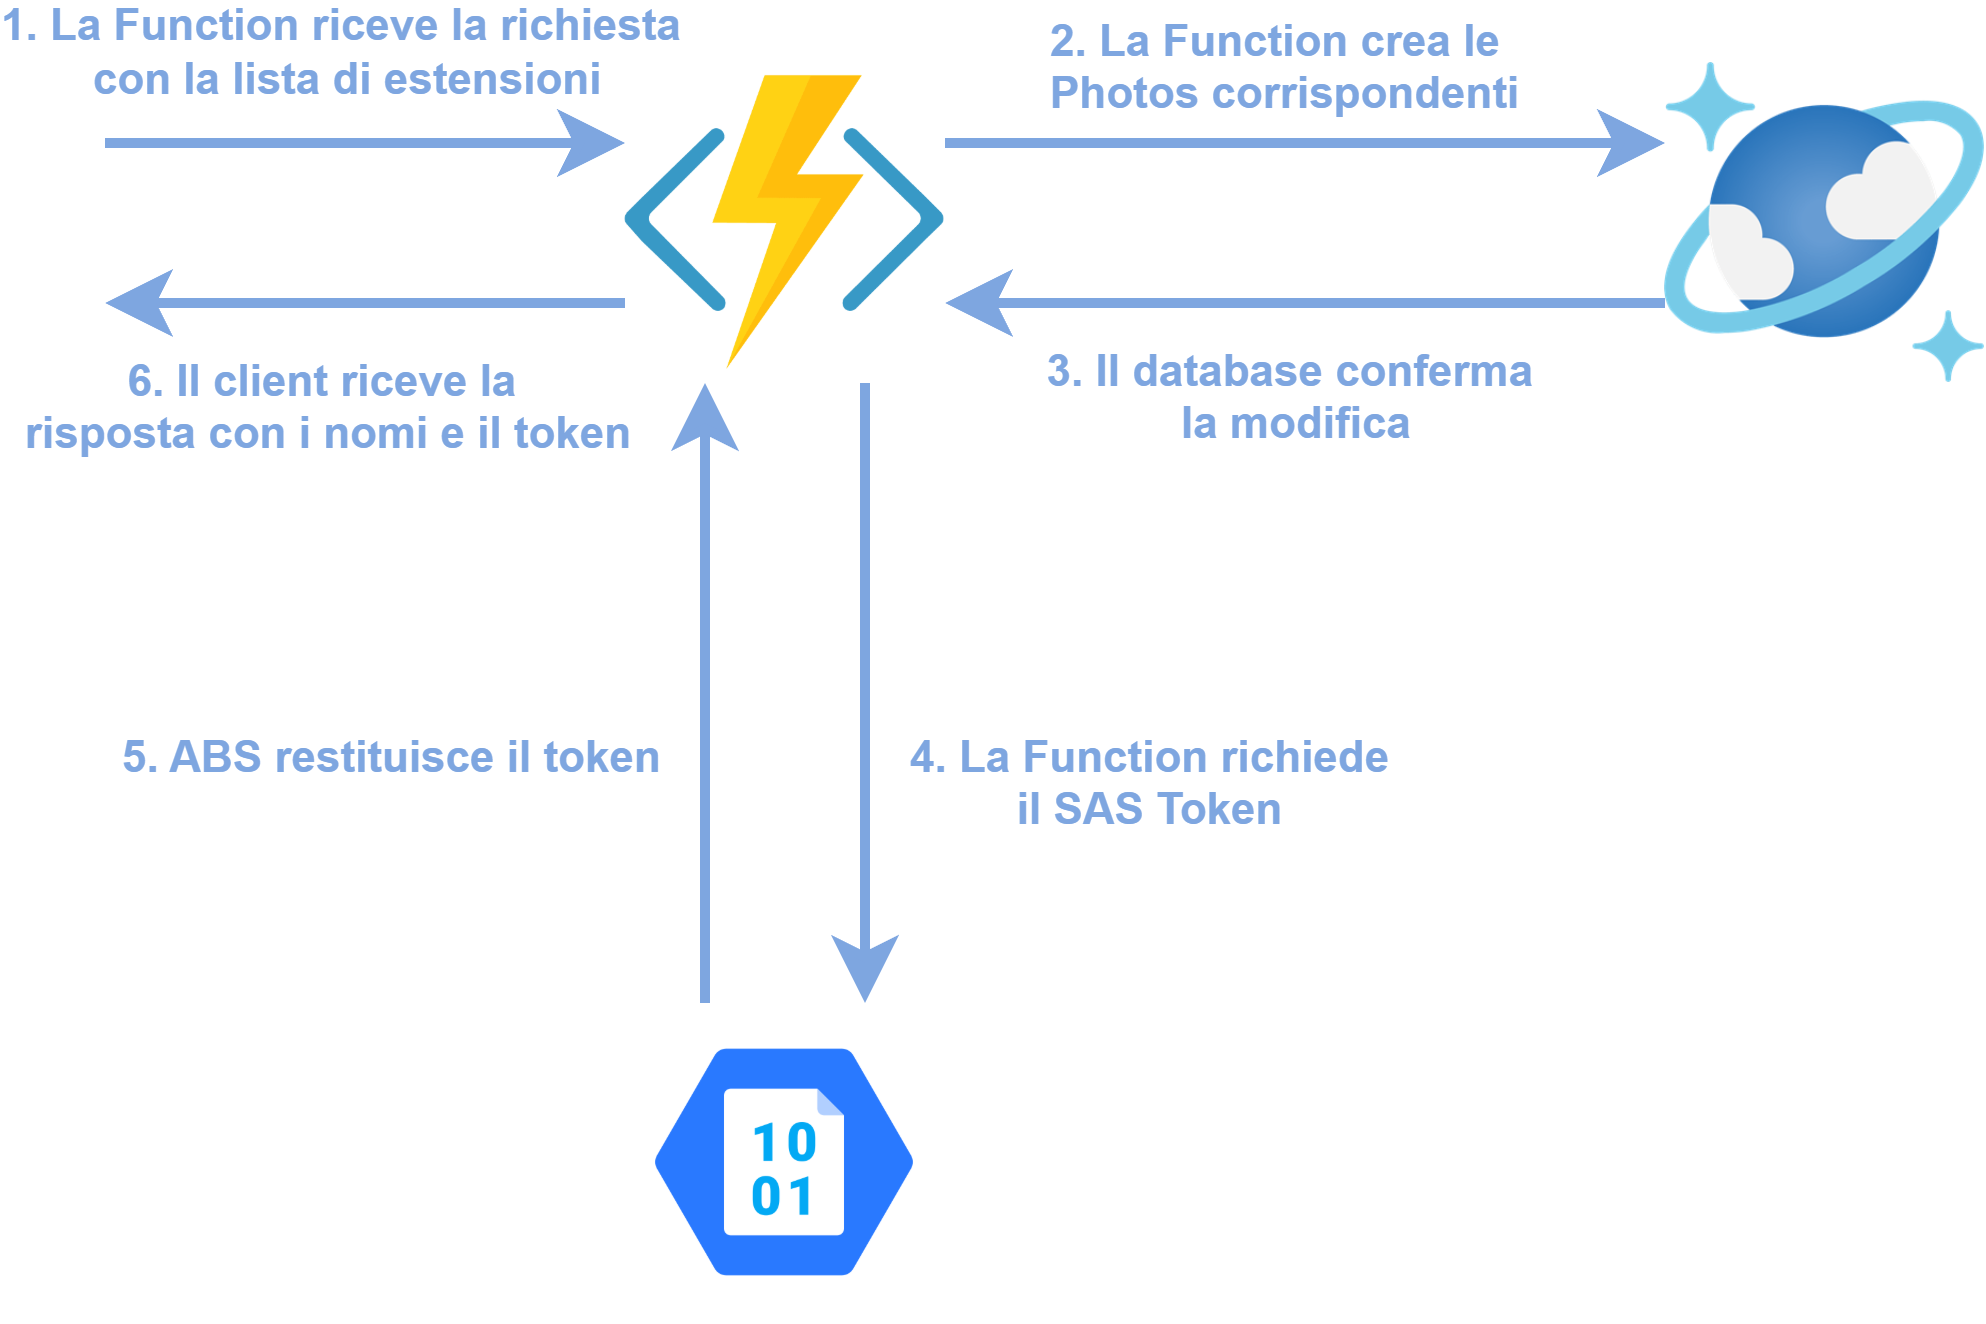
\includegraphics[width=\textwidth]{SASTokenSchema.png}
    \caption{Interazione logica per l'ottenimento del token}
\end{figure}
\\
La risposta verso il client sarà quindi composta, oltre che dal token di accesso, 
anche dai nomi delle immagini, affiancate dalle loro estensioni.
Ricevuta la risposta il client procederà, in simultanea, 
a comprimere i file selezionati, 
per ridurre il consumo di banda e il volume dei dati totali trasmessi.
Questa strategia consente di diminuire il carico computazionale sul server, 
migliorando l’efficienza complessiva del sistema.
Nel momento in cui finisce la procedura di compressione, il device contatterà il Blob Storage e,
usando il SAS token, caricherà le immagini usando il nome associato con l'estensione corretta.\\
\\
La terminazione del caricamento è collegata all'esecuzione di una Azure Function.
Il ruolo di questa funzione è quello di controllare che il file caricato corrisponda
a un'immagine logica sul database.
Controllerà quindi che il nome del file e il percorso associato corrispondano 
al nome dell'immagine e all'evento relativo, 
assicurandosi inoltre che l'estensione non sia cambiata 
e che il suo stato sia lo stesso con cui è stato inizializzato.
In caso uno di questi parametri non coincida, 
procederà eliminando di entrambe le risorse, 
ovvero sia l'immagine logica sul database che il blob caricato.
Altrimenti, se tutto risulta corretto,
procederà ad aggiornare lo stato dell'immagine a "Uploaded".\\
\begin{figure}[h!]
    \centering
    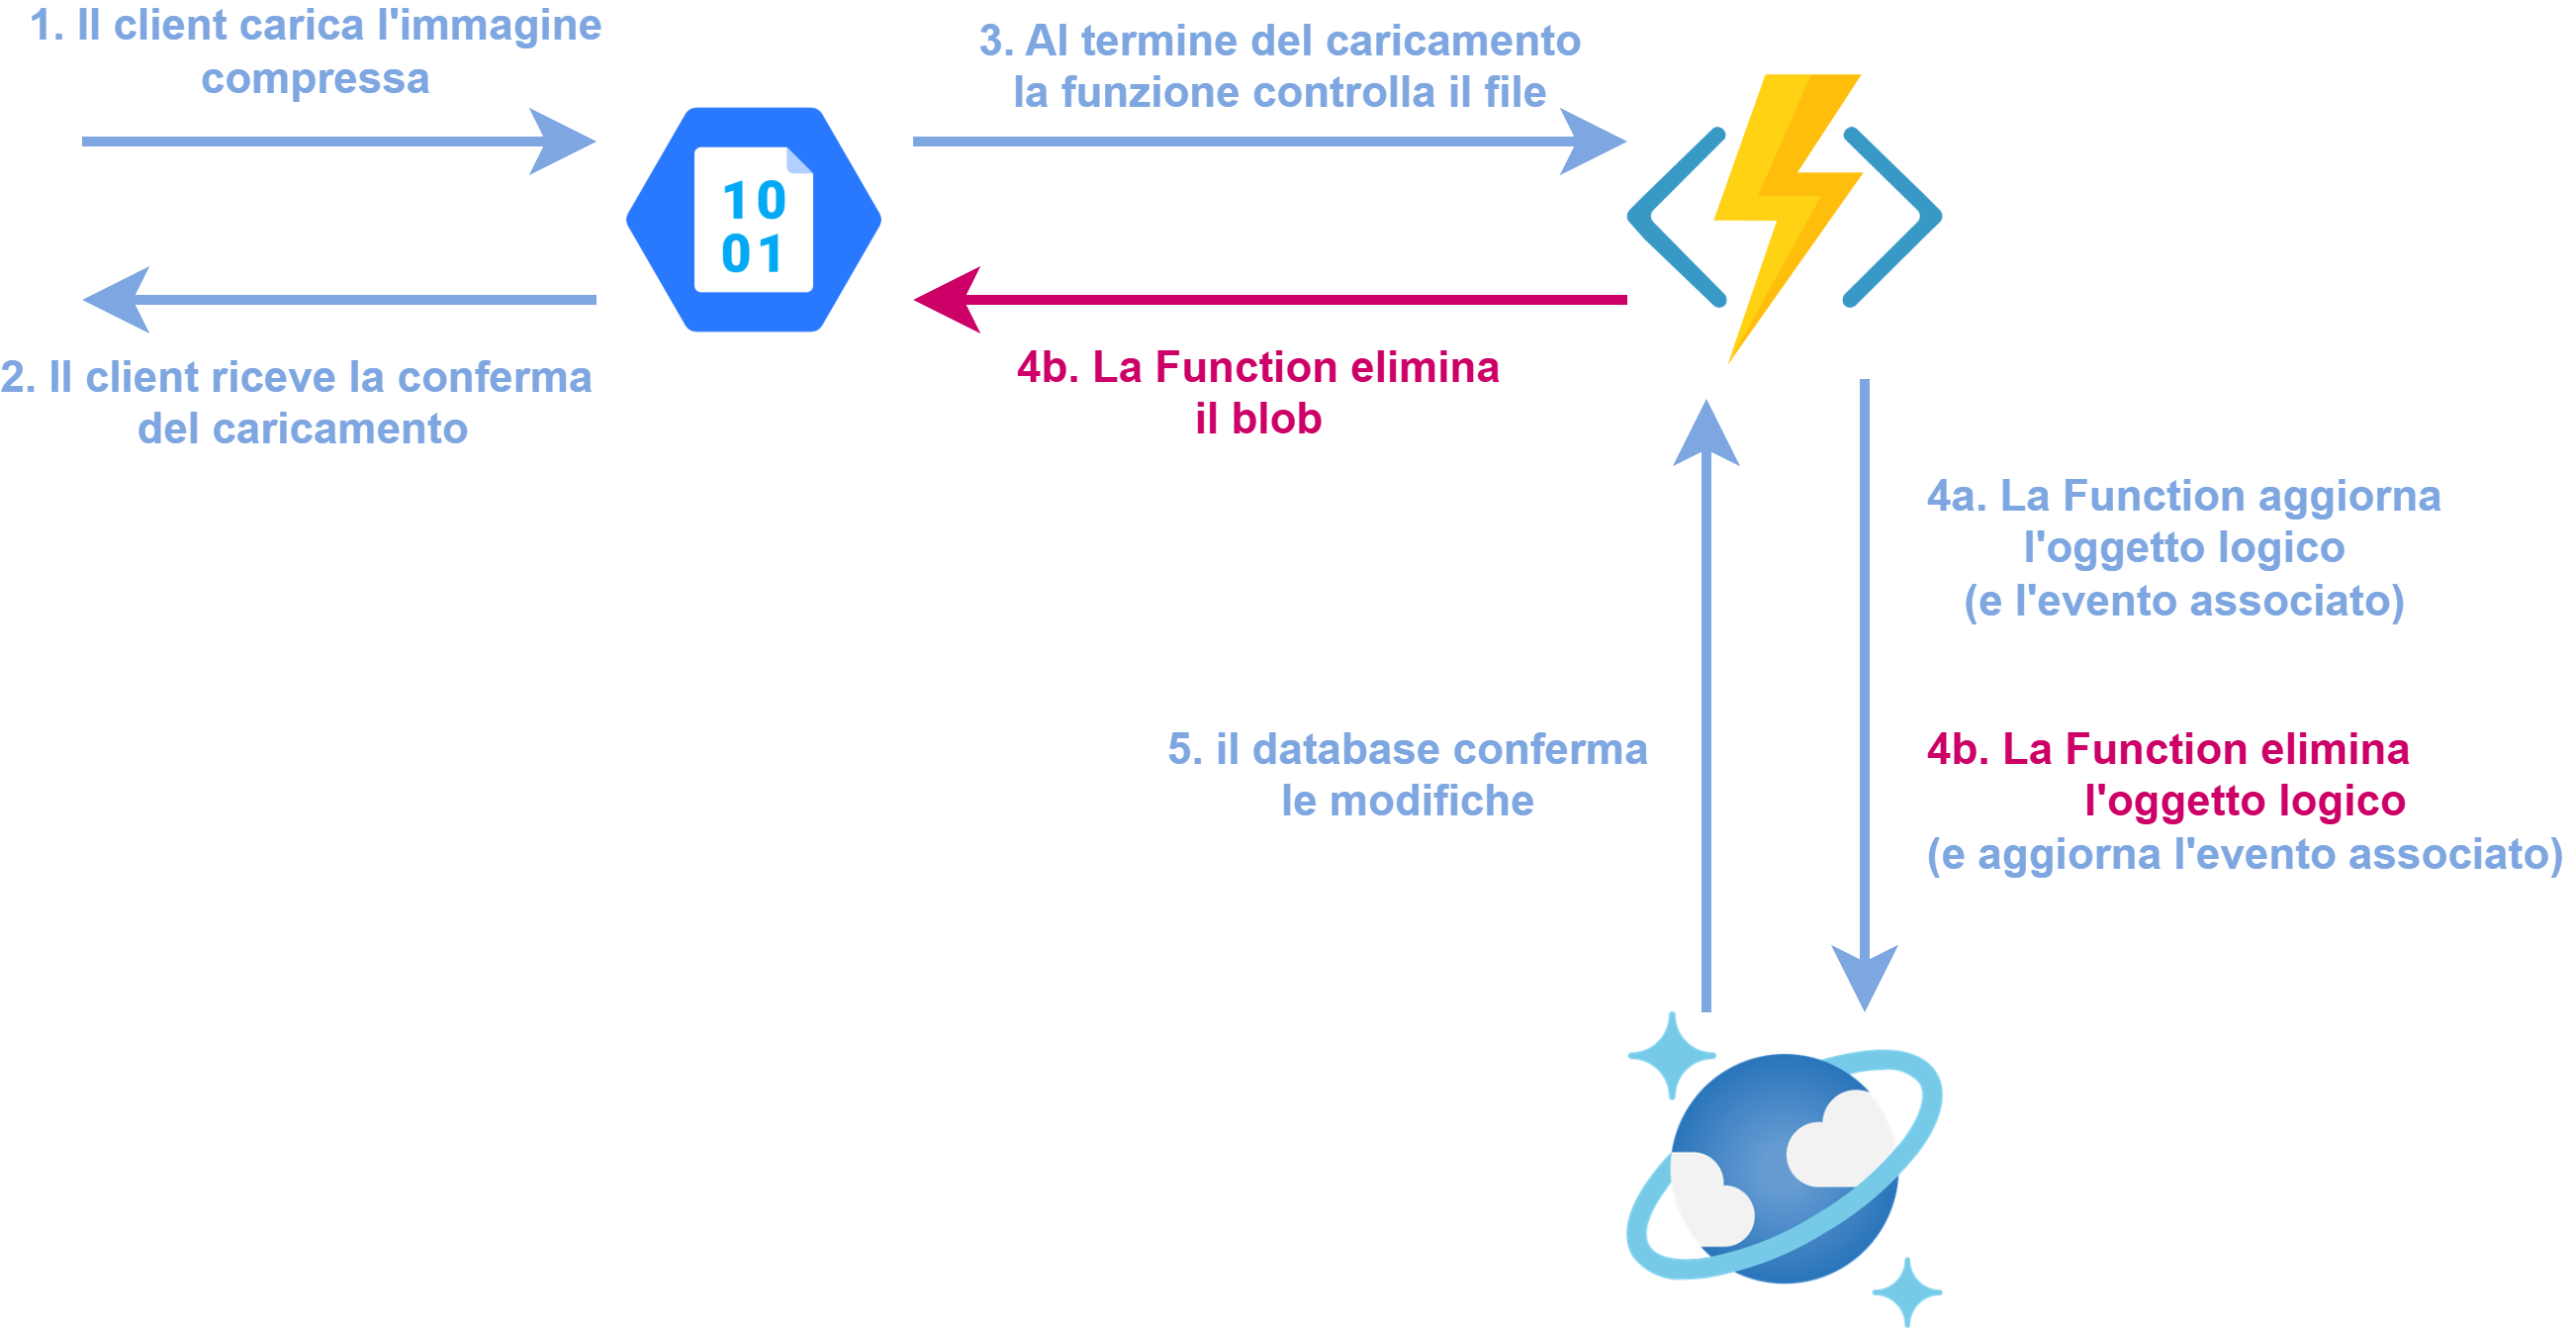
\includegraphics[width=\textwidth]{ImageUploadSchema.png}
    \caption{Interazione logica per il caricamento dell'immagine}
\end{figure}
\\
Il caricamento di un'immagine costituisce una modifica all'evento.
Per questo motivo è necessario aggiornare la data di aggiornamento dell'evento.
Per evitare che troppe richieste ricadano sullo stesso evento,
sarà solo l'ultima funzione chiamata a effettuare la modifica.
A seguito delle operazioni precedenti la funzione controllerà infatti se, 
fra tutte quelle associate all'evento, ci siano immagini con lo stato ancora in "Started".
In caso contrario si deduce che la funzione corrente è l'ultima ad aver effettuato la modifica,
e sarà lei quindi ad aggiornare l'evento relativo.
L'aggiornamento dell'evento comporta la propagazione della notifica a tutti i profili coinvolti.\\
\\
Essendo le immagini così create indipendenti tra loro,
la loro modifica non richiede il blocco o il controllo di altre entità.
Andando a modificare singolarmente le entità logiche delle immagini,
questa operazione risulta altamente parallelizzabile,
garantendo così la scalabilità delle richieste.\\
\\
L'accesso in lettura ai file multimediali in ABS risulta pubblico per impostazione predefinita, 
poiché la mancata definizione di ruoli comporta l'assenza di controlli espliciti sulle autorizzazioni delle richieste. 
Questo aspetto pone delle problematiche sulla privacy delle immagini, 
che viene però mitigato grazie all'uso di hash randomici sufficientemente lunghi, 
che riducono drasticamente la probabilità di collisione. 
Infatti, senza la conoscenza dell'hash corretto, 
un accesso non autorizzato alle immagini 
richiederebbe tentativi casuali estremamente numerosi,
nella speranza di trovare una combinazione corretta, 
rendendo il successo un attacco altamente improbabile. 
Inoltre, anche in caso di compromissione di un hash, 
e quindi la possibilità di recupero di un'immagine da parte di un attore 
il cui accesso non dovrebbe essere permesso,
l'accesso sarebbe limitato a una singola immagine, 
senza fornire ulteriori informazioni sugli altri file memorizzati.
\clearpage